\graphicspath{{./figures}}

\section{Specifications}

For specification definition, further calculations should be done. This will allow a list of more detailed, system-level specifications to be created. First, the required communication conditions (link distance, atmospheric effects etc.) are established. Then, power and voltage requirements are expanded on. Finally, system integration is considered.

Typicall balloon satellites reach a maximum height of around 30 km \cite{site-weatherWeatherBalloons}. They rise at a vertical speed of around 20 km/h, and can travel horizontally as fast as 200 km/h when falling. A typical path distance for such a balloon is 200 km, and therefore an average speed of around 100 km/h will be designed for. This results in an average flight time of longer than 2 hours.

At the above height, a line-of-sight (LOS) calculator reveals that the horizon is around 600 km, meaning that the antenna could theoretically be placed at sea level, assuming no ground obstructions. Further, the earth's curvature is found to be negligible at this distance, meaning pythagoras can be used to calculate a final LOS distance of 120 km. If low-earth orbit (LEO) heights are to be considered as a project expansion, the curvature of the earth should be taken into account. At a height of 160 km, an LOS distance of 1400 km is required, and at 1000 km, an LOS distance of around 3500 km is required. Since this is much further than the required slant range of 120 km, it will not be designed for initially.

\begin{figure}[!htb]
    \centering
    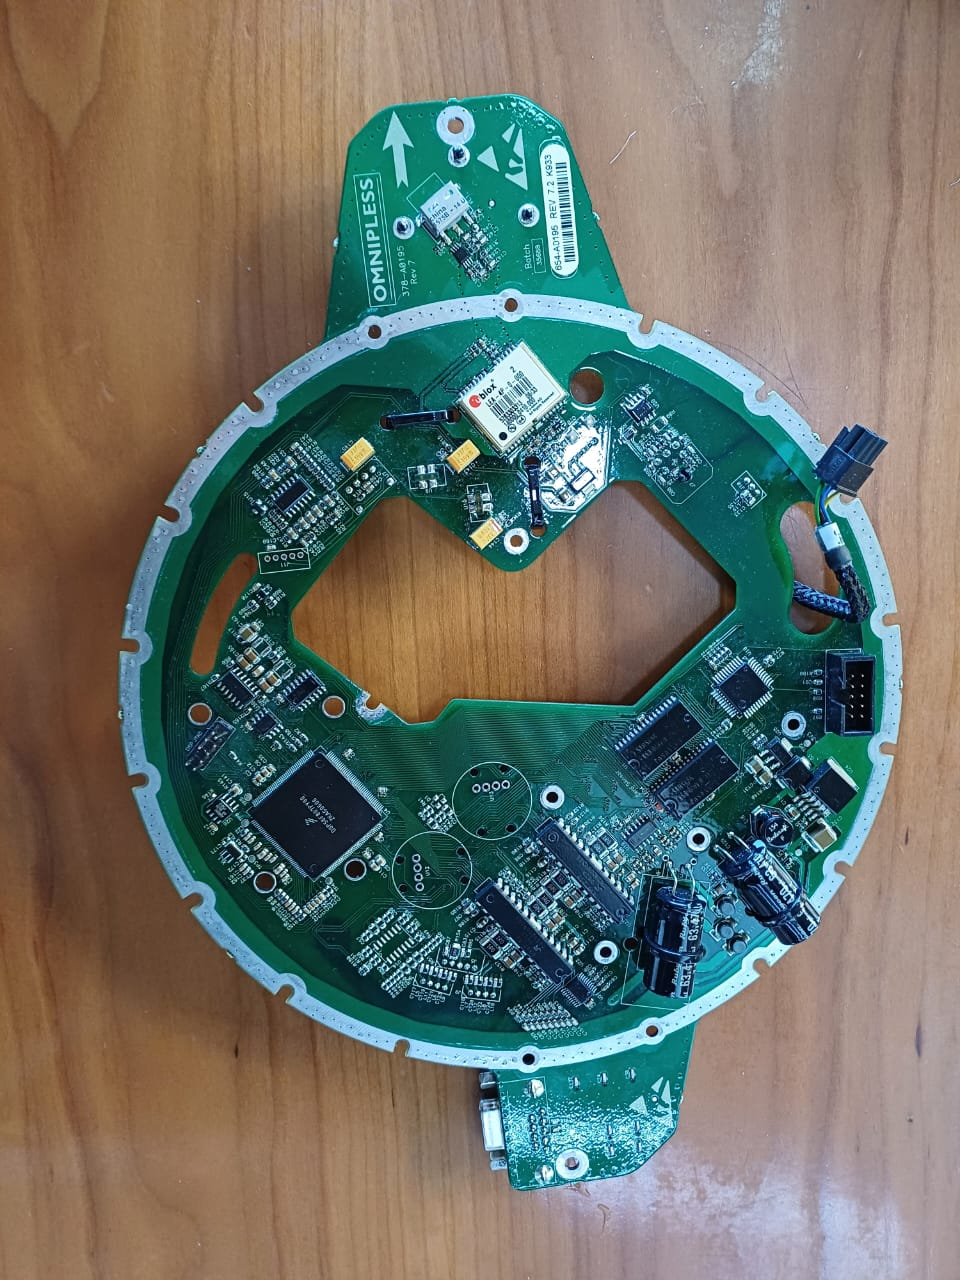
\includegraphics[width=0.4\textwidth, angle=90, origin=c]{gs_existing}
    \caption{Existing Antenna Mount PCB}
    \label{fig:gs_existing}
\end{figure}

The PQSU standard includes 3.3V and 5V bus voltages. One of these must therefore be used directly to power the PQ unit's circuitry. As mentioned, the PQ unit will be integrated with other units into a single PocketQube. Since this is a prototype launch, there is risk of the EPS malfunctioning. Further, a power connection is also needed during development for modularized testing. A simple on-board battery system which matches the standard's voltage will therefore be included in the design to be used for testing and potentially deployment.

The PQSU standard clearly defines the dimensions of a PocketQube PCB (e.g. 42 mm x 42 mm outer dimensions) and the design should conform to this standard. The provided antenna mount allows for an existing circular PCB with mounting holes and two support "wings", as shown in \ref{fig:gs_existing}. The new GS PCB should therefore conform to this form factor. Lastly, the system should drive the stepper motors which are already provided with the antenna mount. The following system-level specifications are therefore drawn up:
\begin{enumerate}
    \item The system should be capable of a slant range of 120 km.
    \item The system should be designed to operate at a minimum data rate of 4800 baud (which the iMet-54 uses \cite{datasheet-iMet54}) or at a target data rate of 9600 baud (which is a typical satellite telemetry downlink speed as in \cite{paper-deployableAntenna}).
    \item The system should allow for iMet-54 radiosonde data to be retreived. This data is GFSK modulated at a pre-selected frequency of between 402 to 405 MHz \cite{datasheet-iMet54}.
    \item A single antenna should be used for both the custom and radiosonde protocol on the GS, to simplify the design. This antenna should therefore have a bandwidth in the range from 405 MHz up to the amateur radio band (433 MHz).
    \item A 100 mW equivalent transmit power restriction should be adhered to.
    \item The PQ unit should follow the PQSU and PQ9 standard, which stipulate:
    \begin{itemize}
        \item A 42 mm square outer PCB dimension
        \item A 4 mm component height above, and a 2 mm component height below.
        \item A 20-pin header interface, catering for RS-485 and I2C communication, and providing 3.3 V and 5 V power lines.
    \end{itemize}
    \item The PQ unit should include a battery capable of lasting 2 hours at nominal current draw.
    \item The GS should be capable of tracking the balloon at 110 km/h, at a line-of-sight distance of 120 km.
    \item The GS PCB should connect to the existing antenna mount, which has a diameter of 198 mm, with equi-spaced mounting holes etc. (as in Figure \ref{fig:gs_existing}).
    \item The GS should control two 4218S-15 bipolar stepper motors, which have a maximum current of 0.50 A per phase, and are driven at 24 V.
    \item The GS should provide a USB-C connection to allow a PC to monitor the telemetry data. This should be capable of receiving all data from the link in realtime.
\end{enumerate}